\section{Data and Event Selection}\label{sec:hmmEvSel}

The search for \hmm is concerned with events containing at least two muons.
This section details the event selection, data, and simulation used in the analysis.

\subsection{Event Selection}\label{sec:hmmEv}

All data events are required to pass several criteria before they are considered for analysis.
Events are considered only if they were recorded while the ATLAS detector was in full operation.
The events meeting this requirement comprise the Good Run List, as summarized in Section \ref{sec:physData}.

Only a small fraction of the many events observed by ATLAS are useful to study. 
The trigger system decides on an event-by-event basis whether to record an event. 
Since \hmm events have muons in their final state, the analysis uses a trigger selection that requires at least one high-\pt muon.
The \pt threshold varies based on the year of data taking, depending on the trigger system's configuration.
In 2015 the minimum threshold was $\pt>20$~GeV, while in other years, it was $\pt>26$~GeV.
Muons with a \pt below 50~GeV are required to have isolated tracks in the ID to reduce the background event rate.
The efficiency of the trigger requirement is $\approx90\%$.

% Object selection
After passing the trigger requirement, the physics objects that comprise the event are tabulated.
The most important objects for leptonic VH \hmm are muons and electrons, but jets and \met are also used to reduce the background.
The definitions of the objects make use of identification and isolation requirements defined in Section \ref{sec:physObjects}.

The muons considered in an event meet the requirements listed in Table \ref{tab:hmmMuonObjSel}.
These can come from the Higgs decay, as well as the leptonic \W and \Z decays.
These are selected to be relatively inclusive due to the rarity of \hmm decays.
All four types of muons are used: CB, CT, ST, SA.
A particularly low \pt threshold of 6~GeV is selected with the four-muon ZH events in mind since one of the four muons often has a low \pt.

% Muons
\begin{table}[H]
    \begin{center}
        \begin{tabular}{ll}
            \toprule
            Type            &CB, CT, ST, SA\\
            Identification  &Loose \\
            Isolation       &FixedCutPflowLoose\\
            $\pt$           &$\pt > 6$~GeV\\
            $\eta$          &$|\eta| < 2.7$\\
            \multirow{2}{*}{Impact parameters}   &$|d_0^{\mathrm{BL}}/\sigma_{d_0^{\mathrm{BL}}}| < 3$\\
            &$|z_0^{\mathrm{PV}}\cdot \sin{\theta}| < 0.5$~mm\\
            \bottomrule
        \end{tabular}
        \caption{Muon selection criteria.}
        \label{tab:hmmMuonObjSel}
    \end{center}
\end{table}

The electrons are considered next, as these are produced by leptonic \W and \Z decays.
With a similar motivation to the muons, this selection is relatively lenient to maximize the selection's efficiency.
Several criteria are included to retain as many prompt electrons as possible while reducing the inclusion of fake electrons.
These are listed in Table \ref{tab:hmmEleObjSel}.

\begin{table}[H]
    \begin{center}
    %\footnotesize
        \begin{tabular}{ll}
            \toprule
            Identification    &Medium LH\\
            Isolation        &FCLoose\\
            $\pt$            &$\pt > 7$~GeV\\
            $\eta$            & $|\eta|<1.37$ or $1.52<|\eta|<2.47$ \\
            Quality            &Not "BADCLUSELECTRON"\\
            \multirow{2}{*}{Impact Parameters}    & $|d_0^{\mathrm{BL}}\ \mathrm{significance}|<5$ \\
            &$|z_0^{\mathrm{PV}} \cdot \sin{\theta}| < 0.5$~mm\\
            \bottomrule
        \end{tabular}
        \caption{Electron selection criteria.}
        \label{tab:hmmEleObjSel}
    \end{center}
\end{table}

Jets are reconstructed in order to remove background events from the VH selection.
The VH leptonic events are expected to produce small jet multiplicities.
Furthermore, jets are used to reduce the presence of ttH events in the selection, by vetoing events that a b-jet.
The criteria for jet selection are given in Table \ref{tab:hmmJetObjSel}.

\begin{table}[H]
    \begin{center}
    %\footnotesize
    \begin{tabular}{ll}
        \toprule
        Algorithm        &AntiKt R=0.4 PFlow\\
        $\eta$            &$|\eta| < 4.5$    \\
        $\pt$            &$\pt > 25$~GeV for $|\eta| < 2.4$, $\pt > 30$~GeV for $2.4 < |\eta| < 4.5$ \\
        % JVT                & $\mathrm{JVT} > 0.59$ for $|\eta| < 2.4$ and 20~GeV$ < \pt < $120~GeV, $\mathrm{JVT} > 0.11$ for $2.4 < |\eta| < 2.5$ and 20~GeV$ < \pt < $120~GeV\\
        \bottomrule
    \end{tabular}
    \caption{Jet selection criteria. Additionally, a combination of track-based variables are used suppress jets from other collisions in the same bunch crossing, called jet-vertex-tagger.\cite{ATLAS-CONF-2014-018}}
    \label{tab:hmmJetObjSel}
    \end{center}
\end{table}

Finally, the missing transverse momentum, \met, is calculated for the event.
The \met is calculated from the \pt of all reconstructed muons, electrons, and tracks not identified with one of these.
This serves as a proxy for the undetected neutrino from leptonic \W decays.

\begin{table}[htp]
\begin{center}
\begin{tabular}{l l l l}
\toprule
Reject & Against & Condition \\
\midrule
\centered{Jet} & \centered{Electron} & \centered{$\Delta(e,\text{jet})R<0.2$} \\ 
\centered{Jet} & \centered{Muon} & \centered{$\Delta(\mu,\text{jet})R<0.2$} \\ 
\centered{Electron} & \centered{Electron} & \centered{lower \pt electron of shared track} \\ 
\centered{Electron} & \centered{Muon} & \centered{share track} \\ 
\centered{Electron} & \centered{Jet} & \centered{$0.2<\Delta(e,\text{jet})R<0.4$} \\ 
\centered{Muon} & \centered{Electron} & \centered{is calo-muon and shares track} \\ 
\centered{Muon} & \centered{Jet} & \centered{$0.2<\Delta(\mu,\text{jet})R<0.4$} \\
\bottomrule
\end{tabular}
\caption{Overlap removal criteria adopted for object selection, applied sequentially. The jet removal against muons is applied for jets satisfying $N_{Trk}(jet)<3$, or ($p_\mathrm{T}^{jet}/p_\mathrm{T}^{\mu}<2$ and $p_\mathrm{T}^{\mu}/\Sigma_{TrkPt}>0.7$)}
\label{tab:hmmOr}
\end{center}
\end{table}

An overlap removal scheme is applied to avoid treating the same detector signature as multiple objects when two objects are reconstructed in close proximity.
This scheme removes objects according to the priorities listed in Table \ref{tab:hmmOr}.

Once the objects within an event have been determined, the next step is to identify events with objects matching the final state of leptonic VH processes.
All events are required at least one oppositely-charged muon pair that can serve as a candidate for \hmm.
Two parallel selections are carried out: 3-lepton events are selected targeting the WH process, while 4-lepton events are selected targeting the ZH process.

In events with two exactly two muons, these are required to be oppositely charged. In events with more than two muons, later charge requirements are applied, as described in table \ref{tab:hmmEv}. The leading $p_T$ muon is required to have $p_T>27$ GeV. The sub-leading $p_T$ muon is required to have $p_T>8$ GeV. The threshold for the sub-leading muon is lowered compared to the ggF/VBF selection to increase the signal yield efficiency. This change, in conjunction with the lower $p_T$ threshold for all muons and the loosening of the opposite charge requirement, increases WH signal yield by 16.9\% and ZH signal yield by 63\%.

Two selections are used to target VH production: a \textbf{3-lepton} category that targets WH production where the W decays leptonically (electrons or muons), and a \textbf{4-lepton} category that targets ZH production where the Z decays leptonically (electrons or muons).
The overall signal efficiency of the WH event selection is 45\%.
The signal efficiency of the ZH event selection is 37\%.
Both of the efficiencies are calculated with respect to the \W/\Z bosons decaying into electrons or muons.

The leptonic VH production does not produce many b-jets, in contrast to the top backgrounds and ttH signal production.
A veto of events containing b-jets helps reduce these backgrounds and also enhances the purity of the signal selection.
Section \ref{sec:expJets} describes how b-jets are identified with several working points that specify the efficiency of identifying a b-jet.
The loosest working point, 85\%, is selected based on its reaction of the background.
Figure \ref{fig:hmmBveto} illustrates signal and background yields in a comparison between vetoes using the 60\% and 85\% working points.
The looser 85\% working point constitutes a stricter veto, and it is seen to reduce the background yields in both the 4-lepton and 3-lepton selections.
The signal yields are not substantially affected.


\begin{figure}[h!]
\captionsetup[subfigure]{position=b}
\centering
\subfloat[][]{{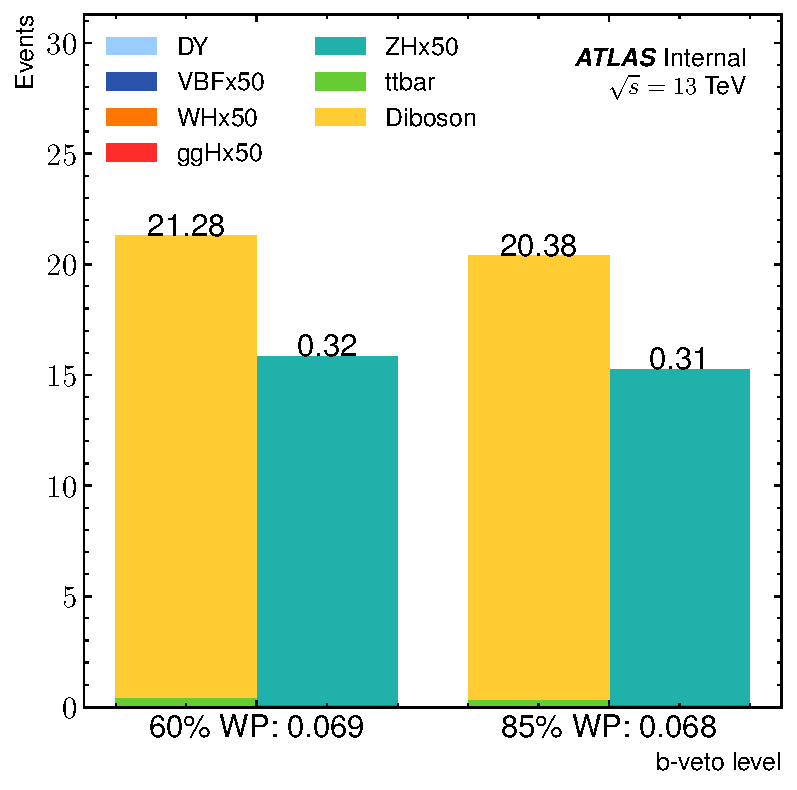
\includegraphics[width=0.5\textwidth]{figures/hmm/bveto/btag-4lep.pdf}}}
\subfloat[][]{{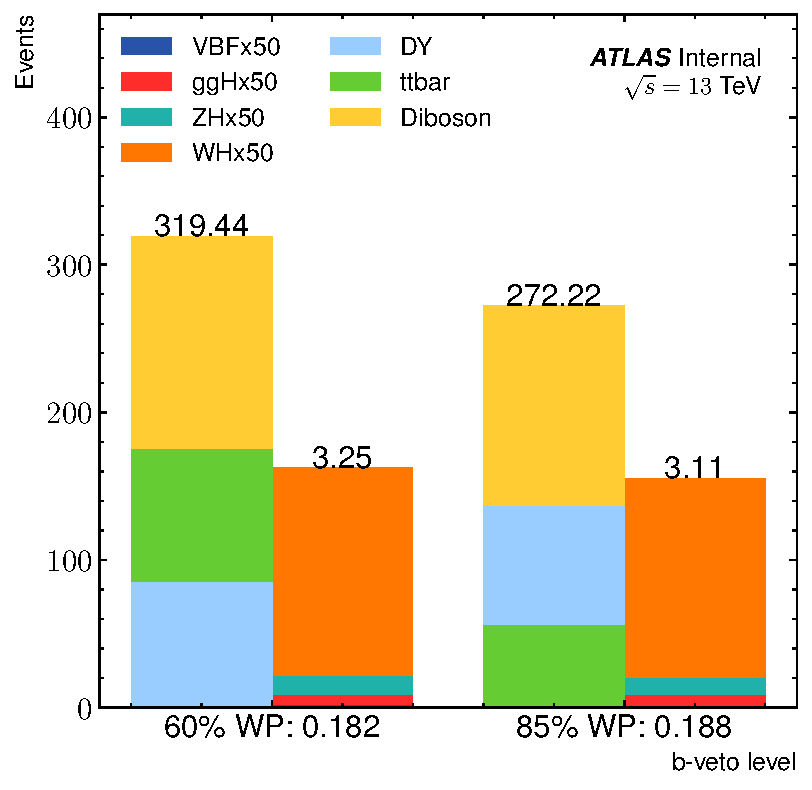
\includegraphics[width=0.5\textwidth]{figures/hmm/bveto/btag-3lep.pdf}}}
\caption{Illustration of the impact on signal and background yields of using different btag working points (WP) for the b-jet veto. This is shown for the 4-lepton selection (a) and 3-lepton selection (b). Each bar shown the number of simulated signal or background events passing the selection when using the WP marked on the x-axis. For both selections, using the looser 85\% WP reduces the background yields compared to the tighter 60\% WP. At the same time, the signal yield is relatively unchanged.}
\label{fig:hmmBveto}
\end{figure}

\begin{table}[ht!]
 \begin{center}
\begin{tabular}{c c  c}\toprule
Step & 4-lepton & 3-lepton \\\midrule
1 & \multicolumn{2}{c}{No 85\% WP btag jets (b-jet veto)}           \\\midrule
2 & At least 4 leptons                                & Exactly 3 leptons\\\midrule
3 & ($N_{\mu^+}>$0 and $N_{\mu^-}>$0)                 & ($N_{\mu^+}>$0 and $N_{\mu^-}>$0) \\\midrule
4 & A dimuon pair $\exists\in$ [110,160] GeV                    & A dimuon pair $\exists\in$ [110,160] GeV \\\midrule
\multirow{2}{*}{5} & ($N_{\mu^+}>$1 and $N_{\mu^-}>$1) or              & ($N_{\mu^+}>$1 or $N_{\mu^-}>$1) or \\
  & ($N_{e^-}>$0 and $N_{e^+}>$0)                    & ($N_{e^-}>$0 or $N_{e^+}>$0)  \\\midrule
6 & $\nexists$ two Z$\to\mu\mu$ candidates                        & $\nexists$ Z$\to\mu\mu$ candidate  \\\midrule
7 & Higgs candidate $\in$ [110,160] GeV                  & Higgs candidate $\in$ [110,160] GeV \\\midrule
\multirow{2}{*}{8} & Kinematic cuts 27/15/8/6 GeV $>p_T$                    & Kinematic cuts 27/10/15(10) GeV $>p_T$ \\
  &                                                        & for $e(\mu)$ \\
\bottomrule\end{tabular}
 \end{center}
 \caption{Cutflow for 4-lepton and 3-lepton selection. Lepton pairs are opposite charge.}
\label{tab:hmmEv}
\end{table}

The steps of the cutflow are shown in table \ref{tab:hmmEv}, which defines the 4-lepton and 3-lepton VH candidate categories.
This cutflow defines ``\Z candidates'' to be oppositely charged dimuon pairs an invariant-mass in $[80,105]$~GeV.
The selection of oppositely charged muons for the Higgs candidate, and of additional leptons for the \Z(\W) candidates is based on minimizing a $\chi^2$ calculation related to the invariant-mass (transverse-mass) of the candidates.
This is shown in equations \ref{eq:hmmWhPairing} and \ref{eq:hmmZhPairing}.
Here, for each candidate pairing, $\chi^{2,\text{cand}}$ is calculated from the Higgs candidate mass $M_H^\text{cand}$.
For 4-lepton events, the \Z candidate mass $M_Z^\text{cand}$ is used, and for 3-lepton events the transverse-mass of the W candidate lepton and $E_T^\text{miss}$, $M_T^\text{cand}$, is used.
Only pairings with oppositely charged muons are considered for $M_H^\text{cand}$, while all oppositely charged same flavor pairs are considered for $M_Z^\text{cand}$.
Leptons of both flavors and charges are considered for $M_T^\text{cand}$.
The pairing with the smallest $\chi^{2,\text{cand}}$ is selected.

\begin{equation}
  \label{eq:hmmWhPairing}
  \chi^{2,\text{cand}} = (M_H^\text{cand}-125\text{ GeV})^2/(3.0\text{ GeV})^2 + (M_T^\text{cand}-70\text{ GeV} )^2/(20\text{ GeV})^2
\end{equation}

\begin{equation}
  \label{eq:hmmZhPairing}
  \chi^{2,\text{cand}} = (M_H^\text{cand}-125\text{ GeV})^2/(3.0\text{ GeV})^2 + (M_Z^\text{cand}-91.1\text{ GeV} )^2/(3\text{ GeV})^2
\end{equation}

The $\chi^2$ pairing is used to improve the pairing efficiency.
Other pairing procedures were considered but were rejected based on their performance.
For example, in 4-muon events, selecting the highest $p_T$ opposite sign muon pair is 63.4\% less efficient than the $\chi^2$ pairing described above. 
Selecting the pair such that the \Z candidate is closest to the \Z mass is 8.7\% less efficient.

The cuts described in table \ref{tab:hmmEv} define two categories of events, 3-lepton and 4-lepton, which are referred to as inclusive categories in relation to the subsequent division into smaller categories.
The kinematic distributions of the leptons in these categories are illustrated in Section \ref{sec:hmmKine}.

\subsection{Simulation}\label{sec:hmmSim}

Simulated datasets play a central role in the search strategy.
All simulated datasets are scaled to match their corresponding cross-section.\cite{CERNYellowReport4}
First, the simulated background and signal datasets allow an exploration of the efficiency of various event selection criteria.
This eventually leads to the criteria listed in Table \ref{tab:hmmEv}.
Next, probability density distributions are constructed from simulated events that describe the probability to observe variables at a given value.
This is done both both for background and signal productions.
This allows the development of a multivariate discriminant function that separates signal and background events based on these variables.
% Simulated events are used at each step of this process: to determine the discriminant function with one set of simulated events and constrain the level of bias it may introduce with a second set of events.
% After this, an unrelated third set is used to estimate the rates of signal and background events, as a function of dimuon invariant mass, at different levels of discrimination.
The background rates as a function of \muu are used to measure systematic uncertainties and to validate the performance of several empirical background models.
The signal shape is used for these purposes as well, and most importantly, it provides the signal component in the hypothesis test performed on the observed data.
Finally, several theoretical and experimental variations on the signal shape are used to measure the impact of these uncertainties on the final result.

% Background ========================
The primary background production in the region of interest comes from Drell-Yan (DY), Diboson, and top production mechanisms described in section \ref{sec:phenoBkg}.
The dominant background mechanism, DY, primarily produces events with two leptons in the final state.
This is reduced through the requirement of more than two leptons in the event selection.
Processes involving $t\tbar$ and single-top production form a large background component as well.
Since the top quark always produces a bottom quark through decay, these backgrounds are mitigated by use of the b-jet veto in the event selection.
After this are diboson productions of $ZZ$ or $WZ$ with leptonic decays.
The diboson is topologically the most similar to the VH signal, making this the most challenging process to reject.
Diboson events are reduced with the help of a discriminant function based on several kinematic observables, but these events remain the dominant background after all selections are complete.

The DY simulations are generated with \sherpa 2.2.1 using the NNPDF3.0 PDF.
The DY \muu spectrum falls exponentially.
To generate sufficient numbers of high-mass events, these are simulated in ranges of $x$, where $x$ is the maximum of the mediator \pt and the scalar parton \pt sum, \httt.
These simulations are produced to NLO for diagrams, including fewer than three jets and LO for diagrams, including three or four jets.

The $t\tbar$ and single-top simulations are produced with \powheg v2 and the NNPDF3.0NLO PDF.
The mass of the top quark is set to $m_t=172.5$.
The $t\tbar$ cross section is calculated to NNLO using Top++2.0. \cite{Czakon:2011xx}
The leading order $t\tbar$ Feynman diagrams are shown in Figure \ref{fig:phenoTtbar}.
The cross-sections of single-top production channels are calculated to NNLL accuracy following the standard procedure. \cite{Kidonakis:2011wy, Kidonakis:2010ux}
The leading order single-top Feynman diagrams are shown in Figure \ref{fig:phenoSingleTop}.
Different simulations are generated for $s$-channel and $t$-channel production through the exchange of a \W boson. A sample is produced for single-top production in association with a \W as well.

The final background simulations are composed of the diboson processes $WZ$ and $ZZ$ with leptonic decays.
These are produced with \sherpa 2.2.1 (for quark decays) and \sherpa 2.2.2 (for fully leptonic decays) and the NNPDF3.0 PDF.
Some number of leptonic decays are needed in order to be interesting for the purpose of the analysis.
One set of simulations simulates $ZZ$\to q\qbar\ll$ and $WZ$\to q\qbar\ll$ events, while a second set simulates events with $\ll\ll$, $\ll\ell\nu$, and $\ll\nu\nu$ final states. \cite{ATL-PHYS-PUB-2017-005}
The purely leptonic $\ll\ll$ originates from two \Z decays.
This is the primary background in the 4-lepton categories and shares a very similar topology to ZH.
For completeness, the $ZZ$ decay to $\ll\nu\nu$ is simulated as well.
The production of $WZ$ $\ll\ell\nu$ is the primary background for several 3-lepton categories.
The leading order diboson Feynman diagrams are shown in Figure \ref{fig:phenoDiboson}.

% Signal simulations ========================
Signal simulations are produced based on the dominant Higgs production mechanisms listed in Table \ref{tab:higgsCrossSec}.
Most simulations are simulated with a Higgs mass set to 125~GeV using \powheg v2 and the PDF4LHC15 PDF. 
The exception is ttH, which is produced with \madgraph and the NNPDF3.0NLO PDF.
The precision ranges from NNLO in QCD for the ggF, to NLO for the VBF, VH, and ttH mechanisms.
The contribution of $gg\to ZH$ is simulated at LO.


\subsection{Kinematic Distributions}\label{sec:hmmKine}

The pre-cut categories defined in Section \ref{sec:hmmEv} are illustrated here with the aid of the simulated signal and background simulations.
The mass distributions are presented in Figure \ref{fig:hmmPrecutMassHists}.
These provide an illustration of the composition of the background and signal contributions to these categories, as well as the general agreement between data and simulation. 

\begin{figure}[h!]
\captionsetup[subfigure]{position=b}
\centering
\subfloat[][]{{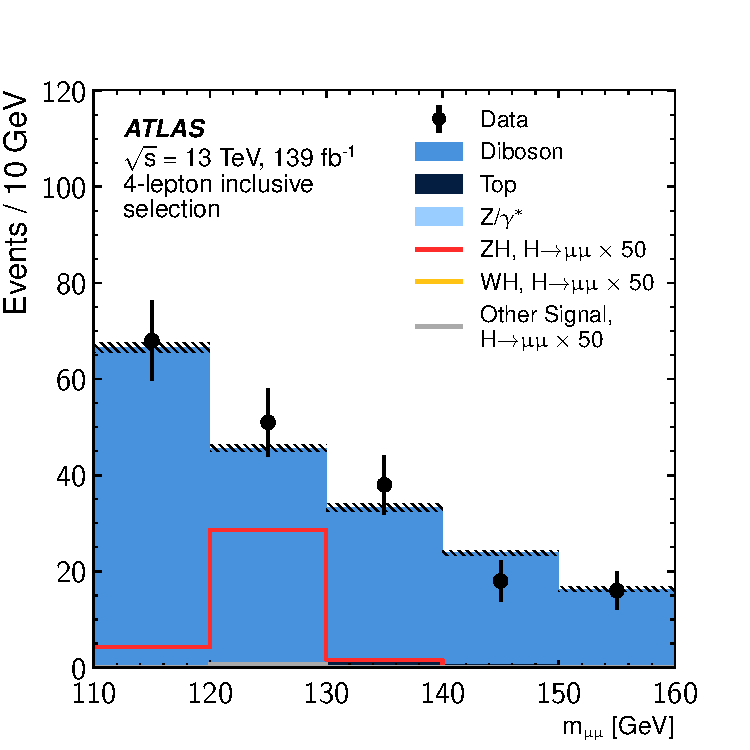
\includegraphics[width=0.5\textwidth]{figures/hmm/public/preCut/histo-4lep-muu.pdf}}}
\subfloat[][]{{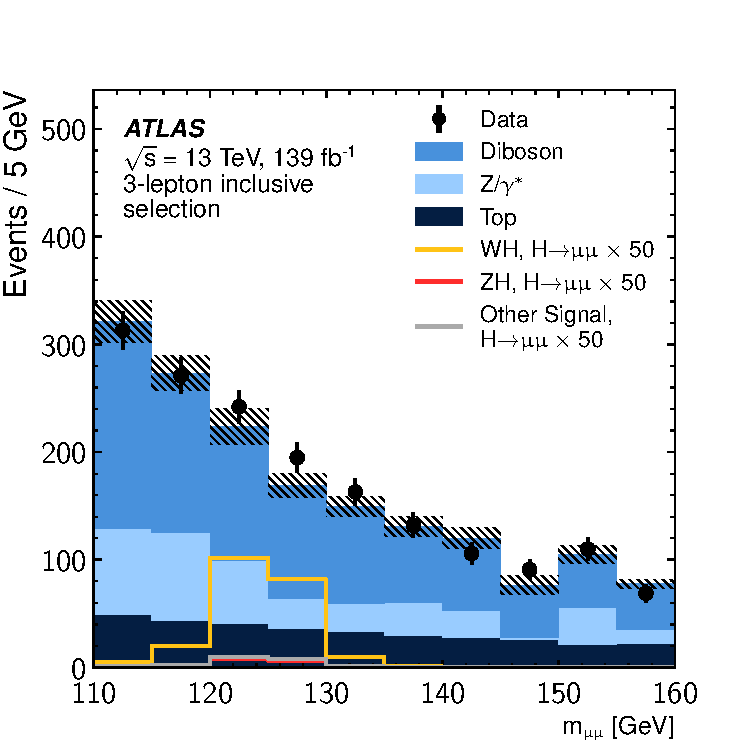
\includegraphics[width=0.5\textwidth]{figures/hmm/public/preCut/histo-3lep-muu.pdf}}}
\caption{Distributions of \muu in the 4-lepton (left) and 3-lepton (right) categories. The binning is adjusted based on the multiplicities of the categories. The signal distributions, shown in colored lines, are scaled by a factor of 50 for visibility.}
\label{fig:hmmPrecutMassHists}
\end{figure}

    
Other kinematic distributions ($p_T$, $\eta$, $\phi$) for the selected leptons are illustrated in Figures \ref{fig:hmmKineWhMuons} to \ref{fig:hmmKineZhLeps}.
The muon candidates for the Higgs are called $\mu^1$ and $\mu^2$ in descending order of $p_T$. 
Likewise, for the 4-lepton category, the selected leptons for the Z candidate are named $\ell^1$ and $\ell^2$ again in descending order of $p_T$.



\clearpage
\begin{figure}[htpb]
  \centering
  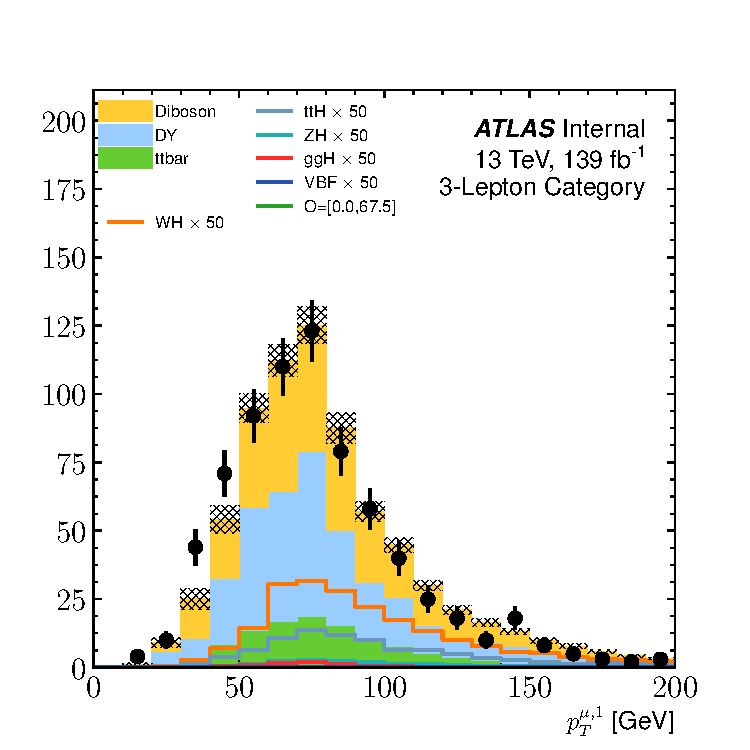
\includegraphics[width=0.4\textwidth]{figures/hmm/kinematics/histo-3lep-u1_pt.pdf}
  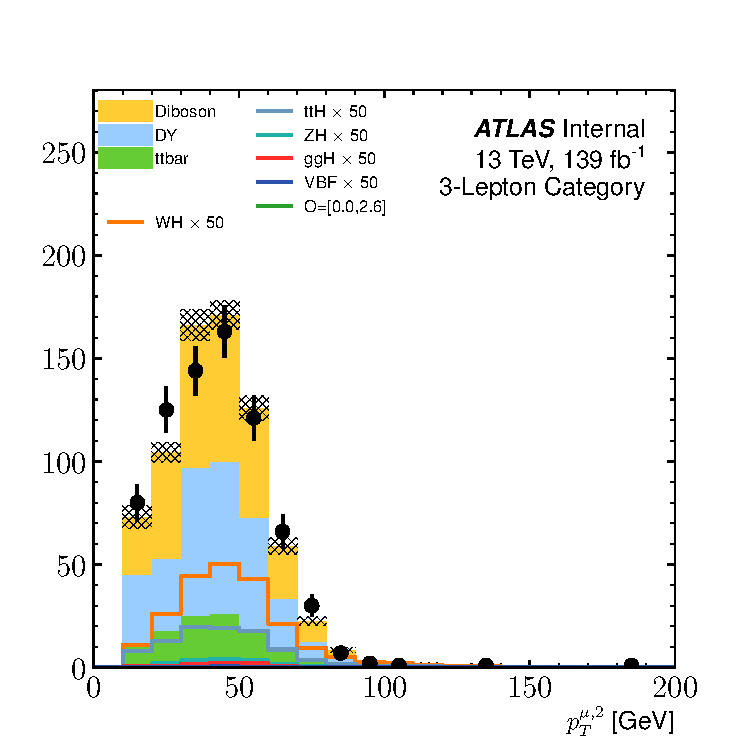
\includegraphics[width=0.4\textwidth]{figures/hmm/kinematics/histo-3lep-u2_pt.pdf}
  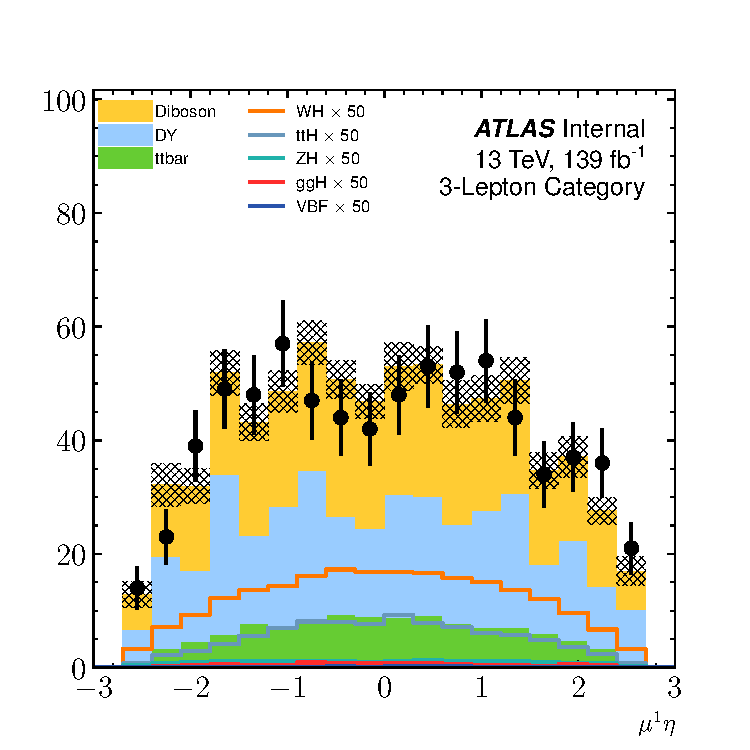
\includegraphics[width=0.4\textwidth]{figures/hmm/kinematics/histo-3lep-u1_eta.pdf}
  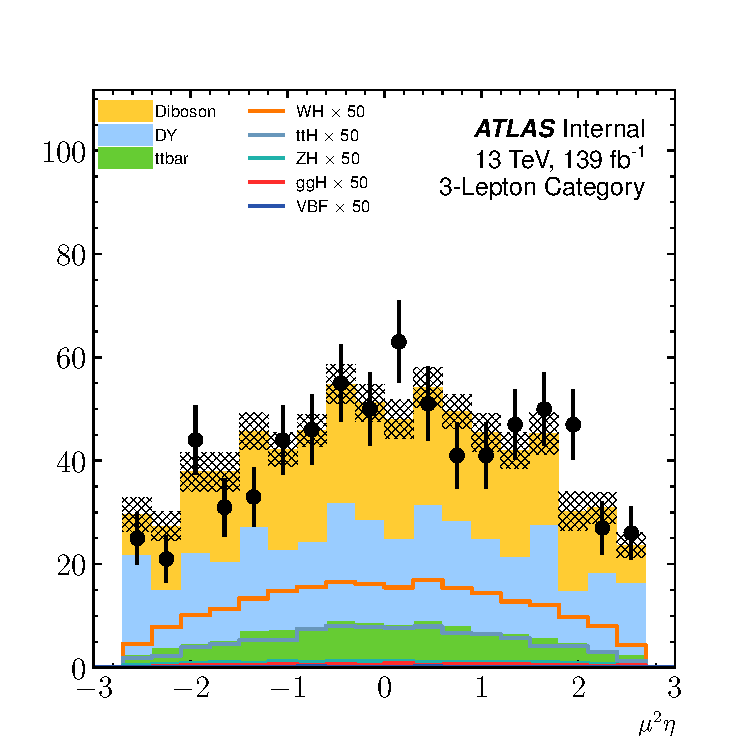
\includegraphics[width=0.4\textwidth]{figures/hmm/kinematics/histo-3lep-u2_eta.pdf}
  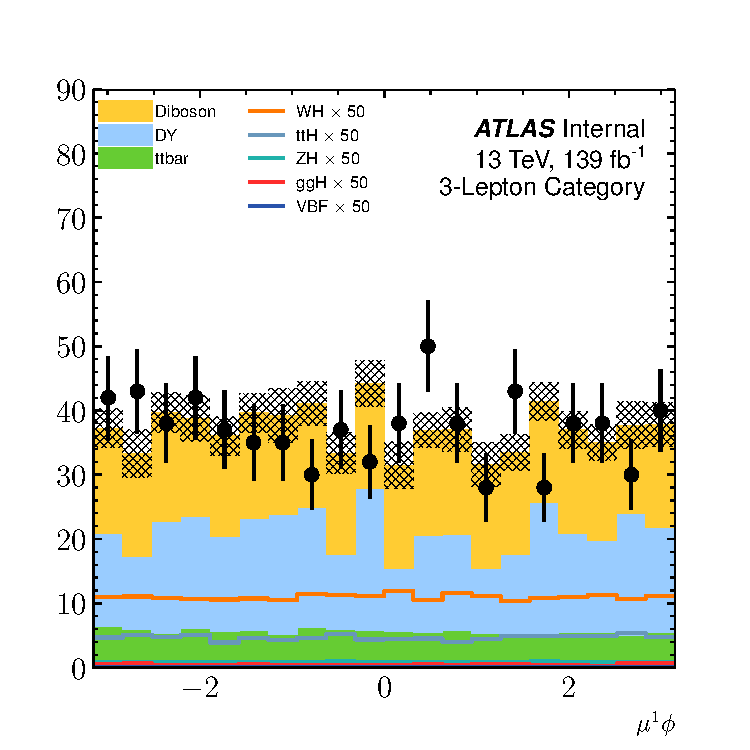
\includegraphics[width=0.4\textwidth]{figures/hmm/kinematics/histo-3lep-u1_phi.pdf}
  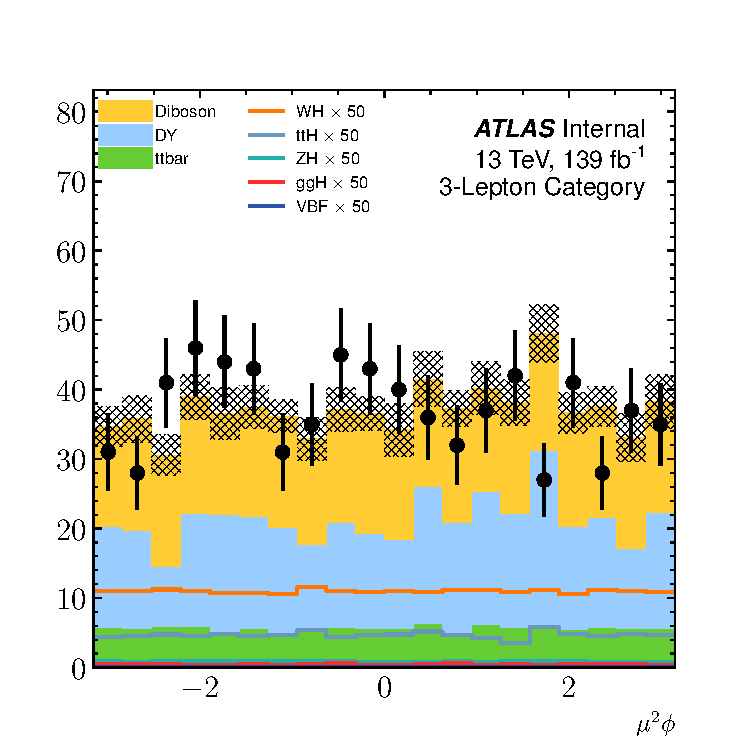
\includegraphics[width=0.4\textwidth]{figures/hmm/kinematics/histo-3lep-u2_phi.pdf}
  \caption{Kinematic plots showing $p_T$, $\eta$, and $\phi$ distributions for the H candidate muons from the 3-lepton selection.}
    \label{fig:hmmKineWhMuons}
\end{figure}

\clearpage
\begin{figure}[htpb]
  \centering
  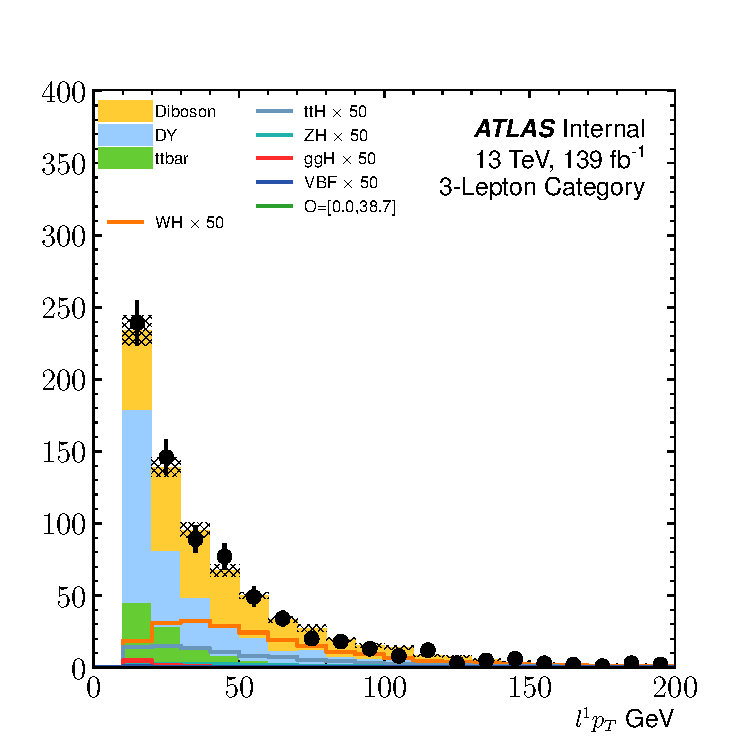
\includegraphics[width=0.4\textwidth]{figures/hmm/kinematics/histo-3lep-aux1_pt.pdf}\\
  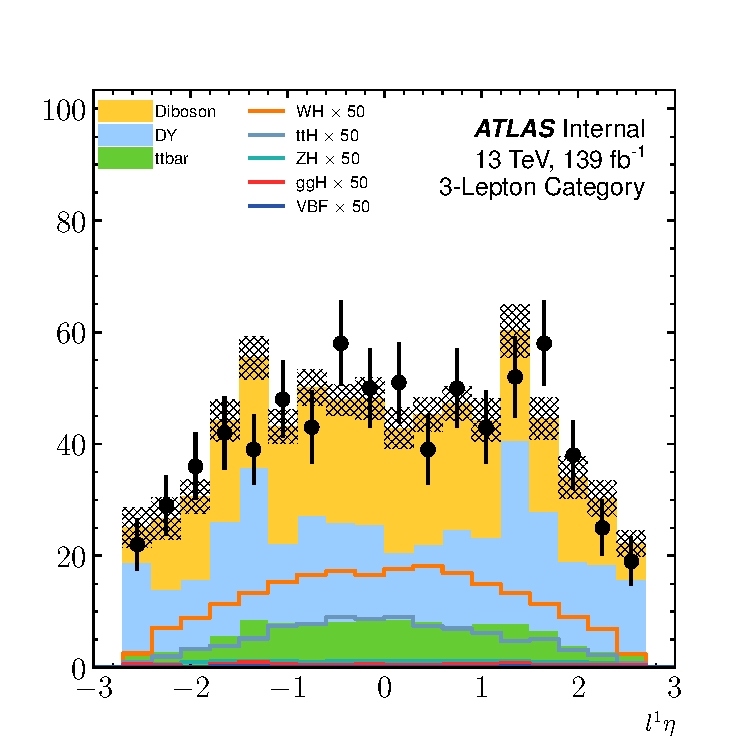
\includegraphics[width=0.4\textwidth]{figures/hmm/kinematics/histo-3lep-aux1_eta.pdf}\\
  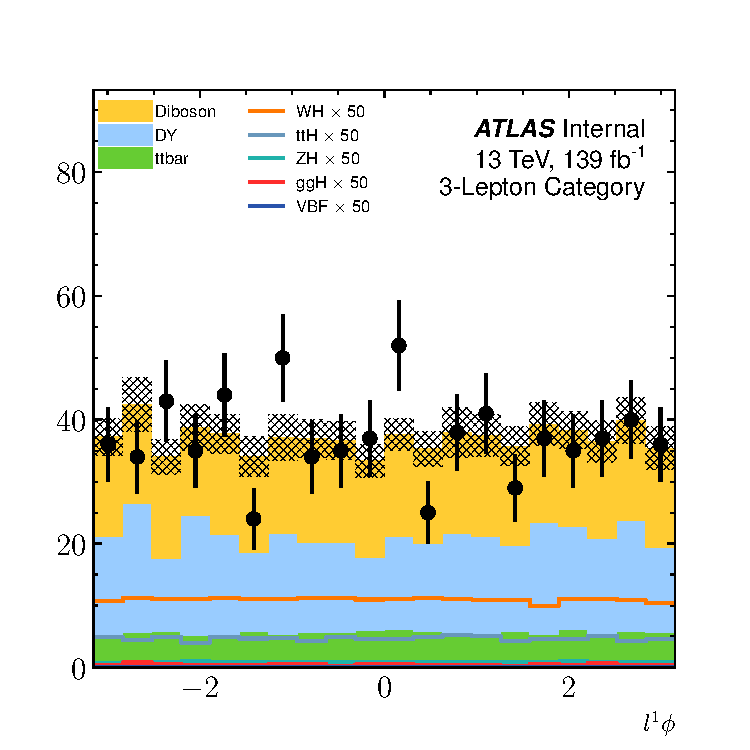
\includegraphics[width=0.4\textwidth]{figures/hmm/kinematics/histo-3lep-aux1_phi.pdf}\\
  \caption{Kinematic plots showing $p_T$, $\eta$, and $\phi$ distributions for the additional lepton/W candidate for the 3-lepton selection.}
    \label{fig:hmmKineWhLeps}
\end{figure}

\clearpage
\begin{figure}[htpb]
  \centering
  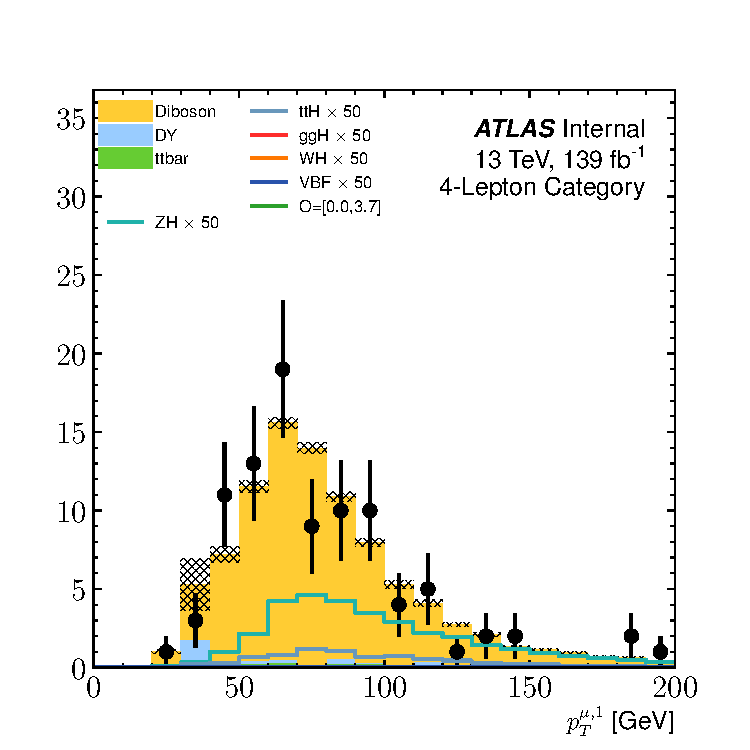
\includegraphics[width=0.4\textwidth]{figures/hmm/kinematics/histo-4lep-u1_pt.pdf}
  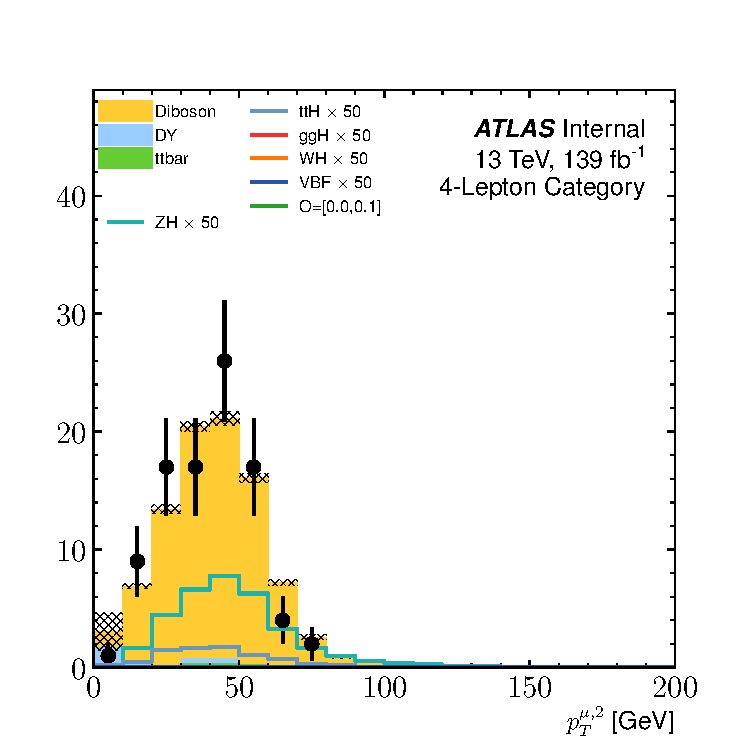
\includegraphics[width=0.4\textwidth]{figures/hmm/kinematics/histo-4lep-u2_pt.pdf}
  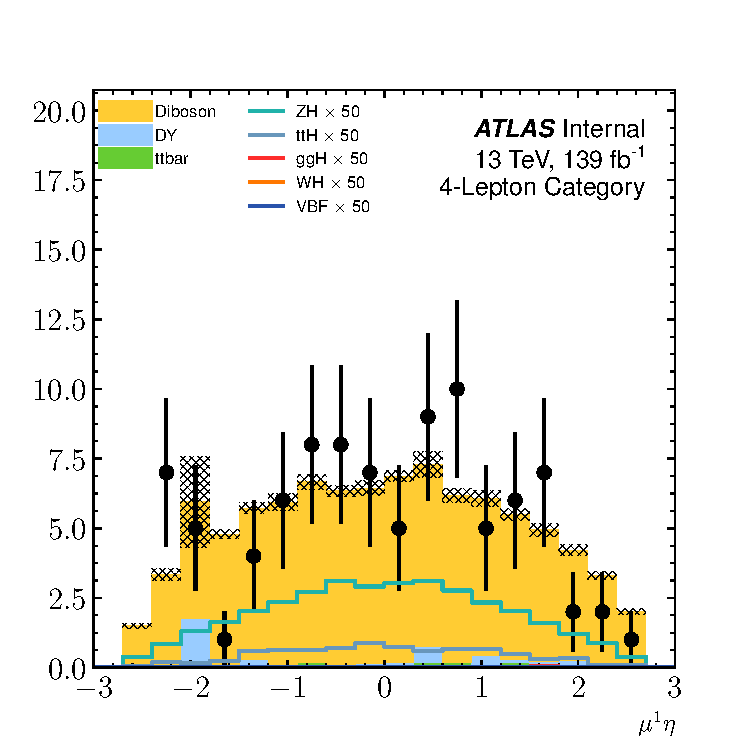
\includegraphics[width=0.4\textwidth]{figures/hmm/kinematics/histo-4lep-u1_eta.pdf}
  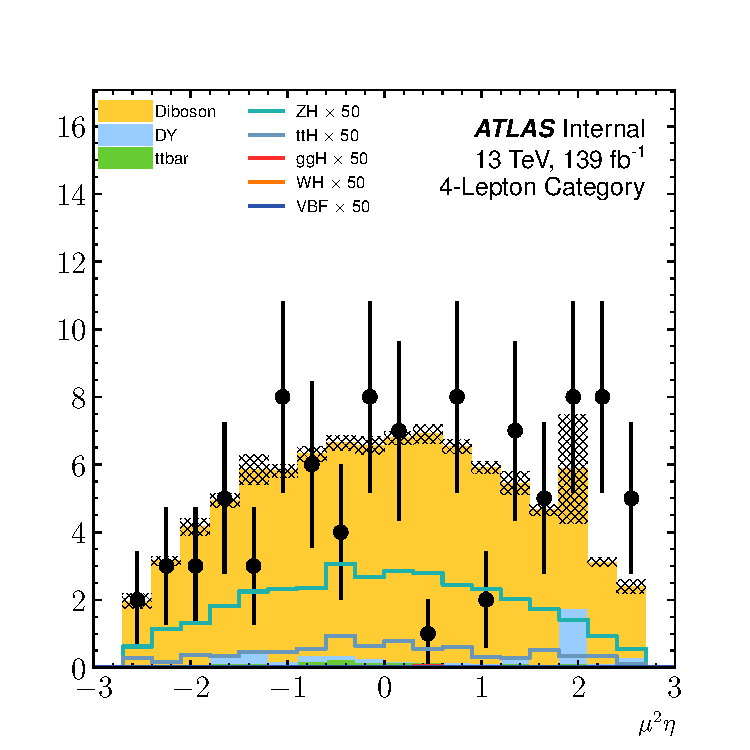
\includegraphics[width=0.4\textwidth]{figures/hmm/kinematics/histo-4lep-u2_eta.pdf}
  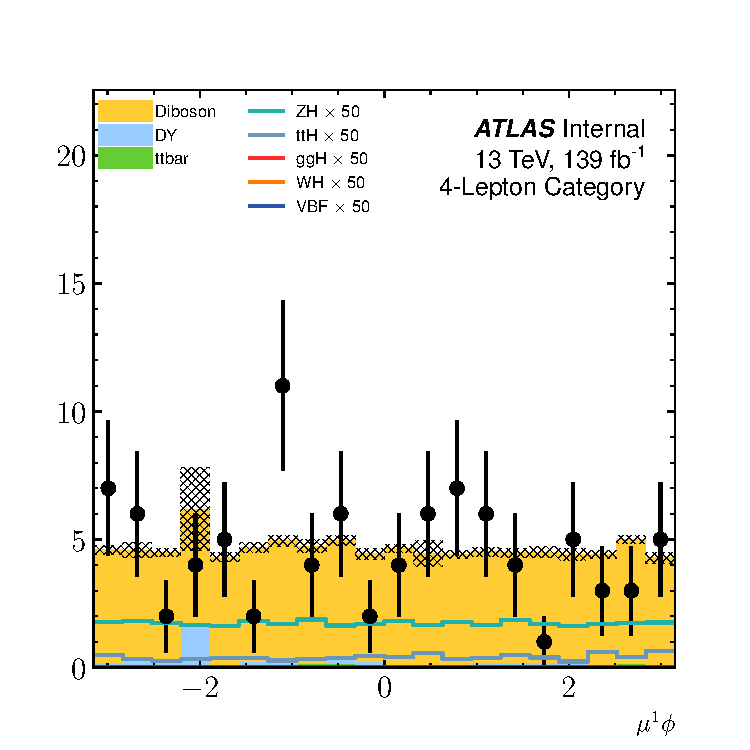
\includegraphics[width=0.4\textwidth]{figures/hmm/kinematics/histo-4lep-u1_phi.pdf}
  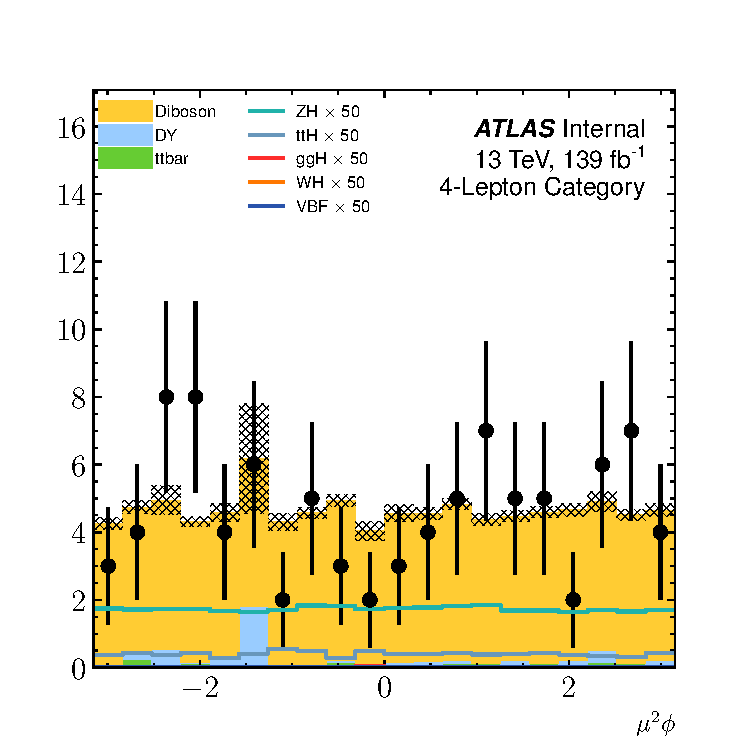
\includegraphics[width=0.4\textwidth]{figures/hmm/kinematics/histo-4lep-u2_phi.pdf}
  \caption{Kinematic plots showing $p_T$, $\eta$, and $\phi$ distributions for the H candidate muons from the 4-lepton selection.}
    \label{fig:hmmKineZhMuons}
\end{figure}

\clearpage
\begin{figure}[htpb]
  \centering
  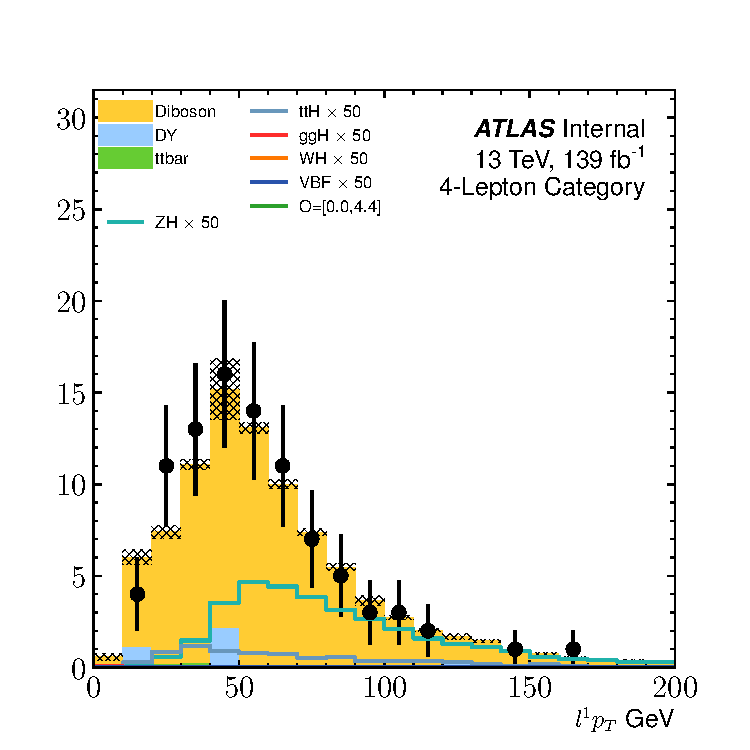
\includegraphics[width=0.4\textwidth]{figures/hmm/kinematics/histo-4lep-aux1_pt.pdf}
  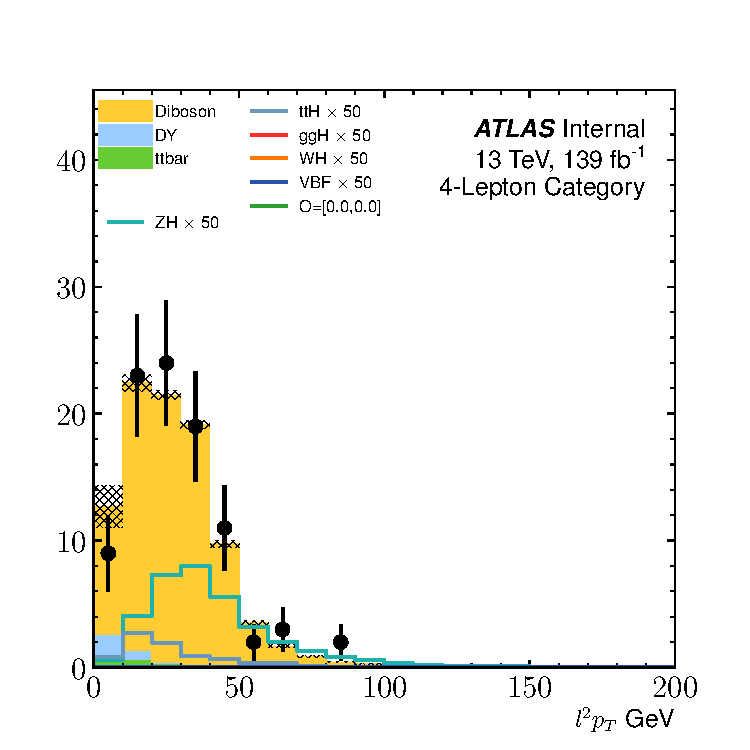
\includegraphics[width=0.4\textwidth]{figures/hmm/kinematics/histo-4lep-aux2_pt.pdf}
  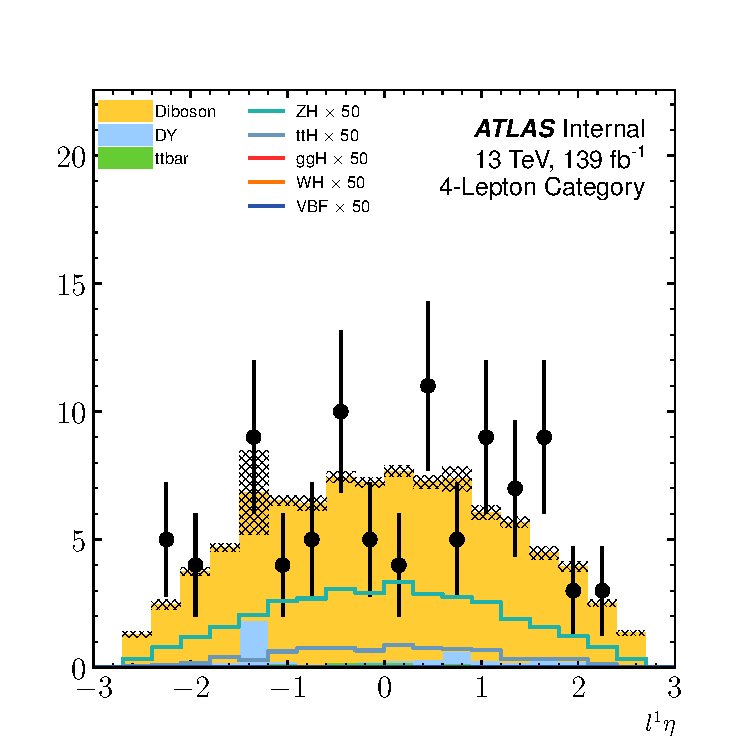
\includegraphics[width=0.4\textwidth]{figures/hmm/kinematics/histo-4lep-aux1_eta.pdf}
  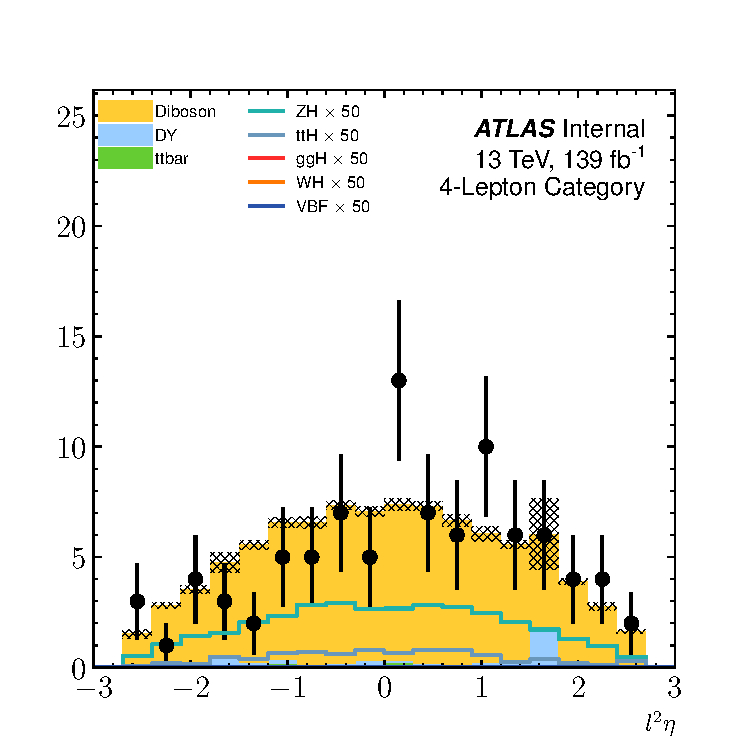
\includegraphics[width=0.4\textwidth]{figures/hmm/kinematics/histo-4lep-aux2_eta.pdf}
  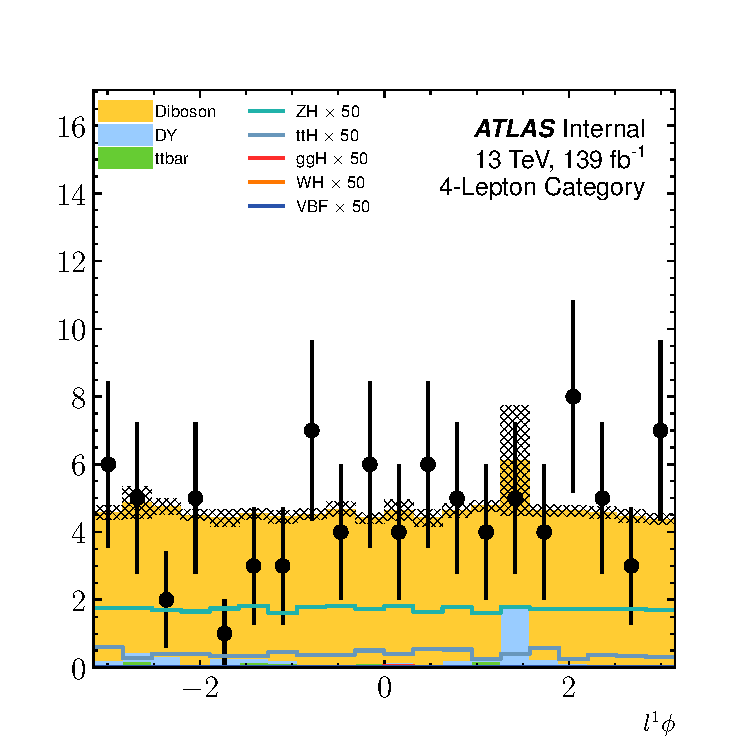
\includegraphics[width=0.4\textwidth]{figures/hmm/kinematics/histo-4lep-aux1_phi.pdf}
  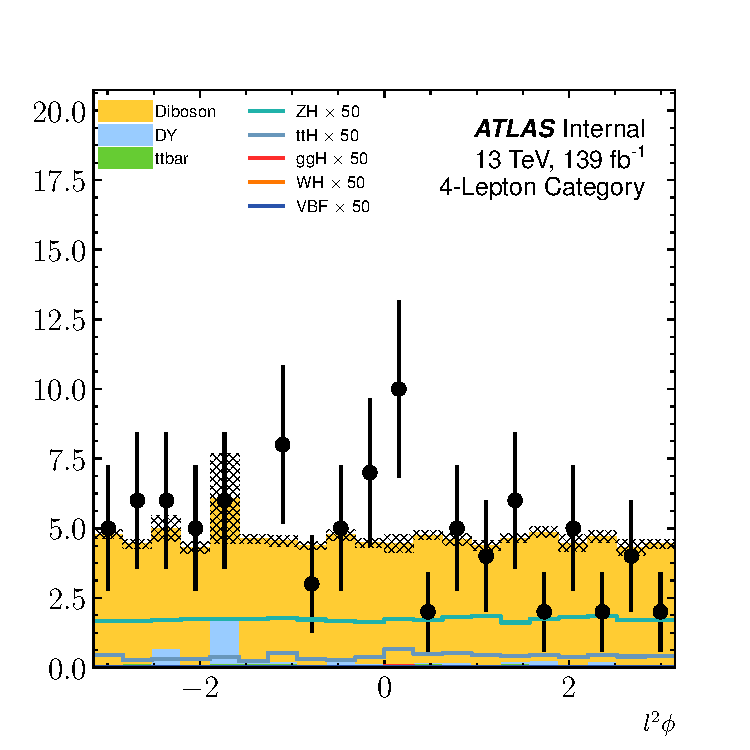
\includegraphics[width=0.4\textwidth]{figures/hmm/kinematics/histo-4lep-aux2_phi.pdf}
  \caption{Kinematic plots showing $p_T$, $\eta$, and $\phi$ distributions for the Z candidate leptons from the 4-lepton selection.}
    \label{fig:hmmKineZhLeps}
\end{figure}
\clearpage


